
%% bare_conf.tex
%% V1.3
%% 2007/01/11
%% by Michael Shell
%% See:
%% http://www.michaelshell.org/
%% for current contact information.
%%
%% This is a skeleton file demonstrating the use of IEEEtran.cls
%% (requires IEEEtran.cls version 1.7 or later) with an IEEE conference paper.
%%
%% Support sites:
%% http://www.michaelshell.org/tex/ieeetran/
%% http://www.ctan.org/tex-archive/macros/latex/contrib/IEEEtran/
%% and
%% http://www.ieee.org/

%%*************************************************************************
%% Legal Notice:
%% This code is offered as-is without any warranty either expressed or
%% implied; without even the implied warranty of MERCHANTABILITY or
%% FITNESS FOR A PARTICULAR PURPOSE! 
%% User assumes all risk.
%% In no event shall IEEE or any contributor to this code be liable for
%% any damages or losses, including, but not limited to, incidental,
%% consequential, or any other damages, resulting from the use or misuse
%% of any information contained here.
%%
%% All comments are the opinions of their respective authors and are not
%% necessarily endorsed by the IEEE.
%%
%% This work is distributed under the LaTeX Project Public License (LPPL)
%% ( http://www.latex-project.org/ ) version 1.3, and may be freely used,
%% distributed and modified. A copy of the LPPL, version 1.3, is included
%% in the base LaTeX documentation of all distributions of LaTeX released
%% 2003/12/01 or later.
%% Retain all contribution notices and credits.
%% ** Modified files should be clearly indicated as such, including  **
%% ** renaming them and changing author support contact information. **
%%
%% File list of work: IEEEtran.cls, IEEEtran_HOWTO.pdf, bare_adv.tex,
%%                    bare_conf.tex, bare_jrnl.tex, bare_jrnl_compsoc.tex
%%*************************************************************************

% *** Authors should verify (and, if needed, correct) their LaTeX system  ***
% *** with the testflow diagnostic prior to trusting their LaTeX platform ***
% *** with production work. IEEE's font choices can trigger bugs that do  ***
% *** not appear when using other class files.                            ***
% The testflow support page is at:
% http://www.michaelshell.org/tex/testflow/



% Note that the a4paper option is mainly intended so that authors in
% countries using A4 can easily print to A4 and see how their papers will
% look in print - the typesetting of the document will not typically be
% affected with changes in paper size (but the bottom and side margins will).
% Use the testflow package mentioned above to verify correct handling of
% both paper sizes by the user's LaTeX system.
%
% Also note that the "draftcls" or "draftclsnofoot", not "draft", option
% should be used if it is desired that the figures are to be displayed in
% draft mode.
%
\documentclass[conference]{IEEEtran}
% Add the compsoc option for Computer Society conferences.
%
% If IEEEtran.cls has not been installed into the LaTeX system files,
% manually specify the path to it like:
% \documentclass[conference]{../sty/IEEEtran}





% Some very useful LaTeX packages include:
% (uncomment the ones you want to load)


% *** MISC UTILITY PACKAGES ***
%
%\usepackage{ifpdf}
% Heiko Oberdiek's ifpdf.sty is very useful if you need conditional
% compilation based on whether the output is pdf or dvi.
% usage:
% \ifpdf
%   % pdf code
% \else
%   % dvi code
% \fi
% The latest version of ifpdf.sty can be obtained from:
% http://www.ctan.org/tex-archive/macros/latex/contrib/oberdiek/
% Also, note that IEEEtran.cls V1.7 and later provides a builtin
% \ifCLASSINFOpdf conditional that works the same way.
% When switching from latex to pdflatex and vice-versa, the compiler may
% have to be run twice to clear warning/error messages.






% *** CITATION PACKAGES ***
%
\usepackage{cite}
% cite.sty was written by Donald Arseneau
% V1.6 and later of IEEEtran pre-defines the format of the cite.sty package
% \cite{} output to follow that of IEEE. Loading the cite package will
% result in citation numbers being automatically sorted and properly
% "compressed/ranged". e.g., [1], [9], [2], [7], [5], [6] without using
% cite.sty will become [1], [2], [5]--[7], [9] using cite.sty. cite.sty's
% \cite will automatically add leading space, if needed. Use cite.sty's
% noadjust option (cite.sty V3.8 and later) if you want to turn this off.
% cite.sty is already installed on most LaTeX systems. Be sure and use
% version 4.0 (2003-05-27) and later if using hyperref.sty. cite.sty does
% not currently provide for hyperlinked citations.
% The latest version can be obtained at:
% http://www.ctan.org/tex-archive/macros/latex/contrib/cite/
% The documentation is contained in the cite.sty file itself.


\usepackage{graphicx}

\usepackage{float}
\floatstyle{boxed}
\restylefloat{figure}

% *** GRAPHICS RELATED PACKAGES ***
%
\ifCLASSINFOpdf
  % \usepackage[pdftex]{graphicx}
  % declare the path(s) where your graphic files are
  % \graphicspath{{../pdf/}{../jpeg/}}
  % and their extensions so you won't have to specify these with
  % every instance of \includegraphics
  % \DeclareGraphicsExtensions{.pdf,.jpeg,.png}
\else
  % or other class option (dvipsone, dvipdf, if not using dvips). graphicx
  % will default to the driver specified in the system graphics.cfg if no
  % driver is specified.
  % \usepackage[dvips]{graphicx}
  % declare the path(s) where your graphic files are
  % \graphicspath{{../eps/}}
  % and their extensions so you won't have to specify these with
  % every instance of \includegraphics
  % \DeclareGraphicsExtensions{.eps}
\fi
% graphicx was written by David Carlisle and Sebastian Rahtz. It is
% required if you want graphics, photos, etc. graphicx.sty is already
% installed on most LaTeX systems. The latest version and documentation can
% be obtained at: 
% http://www.ctan.org/tex-archive/macros/latex/required/graphics/
% Another good source of documentation is "Using Imported Graphics in
% LaTeX2e" by Keith Reckdahl which can be found as epslatex.ps or
% epslatex.pdf at: http://www.ctan.org/tex-archive/info/
%
% latex, and pdflatex in dvi mode, support graphics in encapsulated
% postscript (.eps) format. pdflatex in pdf mode supports graphics
% in .pdf, .jpeg, .png and .mps (metapost) formats. Users should ensure
% that all non-photo figures use a vector format (.eps, .pdf, .mps) and
% not a bitmapped formats (.jpeg, .png). IEEE frowns on bitmapped formats
% which can result in "jaggedy"/blurry rendering of lines and letters as
% well as large increases in file sizes.
%
% You can find documentation about the pdfTeX application at:
% http://www.tug.org/applications/pdftex





% *** MATH PACKAGES ***
%
%\usepackage[cmex10]{amsmath}
% A popular package from the American Mathematical Society that provides
% many useful and powerful commands for dealing with mathematics. If using
% it, be sure to load this package with the cmex10 option to ensure that
% only type 1 fonts will utilized at all point sizes. Without this option,
% it is possible that some math symbols, particularly those within
% footnotes, will be rendered in bitmap form which will result in a
% document that can not be IEEE Xplore compliant!
%
% Also, note that the amsmath package sets \interdisplaylinepenalty to 10000
% thus preventing page breaks from occurring within multiline equations. Use:
%\interdisplaylinepenalty=2500
% after loading amsmath to restore such page breaks as IEEEtran.cls normally
% does. amsmath.sty is already installed on most LaTeX systems. The latest
% version and documentation can be obtained at:
% http://www.ctan.org/tex-archive/macros/latex/required/amslatex/math/





% *** SPECIALIZED LIST PACKAGES ***
%
%\usepackage{algorithmic}
% algorithmic.sty was written by Peter Williams and Rogerio Brito.
% This package provides an algorithmic environment fo describing algorithms.
% You can use the algorithmic environment in-text or within a figure
% environment to provide for a floating algorithm. Do NOT use the algorithm
% floating environment provided by algorithm.sty (by the same authors) or
% algorithm2e.sty (by Christophe Fiorio) as IEEE does not use dedicated
% algorithm float types and packages that provide these will not provide
% correct IEEE style captions. The latest version and documentation of
% algorithmic.sty can be obtained at:
% http://www.ctan.org/tex-archive/macros/latex/contrib/algorithms/
% There is also a support site at:
% http://algorithms.berlios.de/index.html
% Also of interest may be the (relatively newer and more customizable)
% algorithmicx.sty package by Szasz Janos:
% http://www.ctan.org/tex-archive/macros/latex/contrib/algorithmicx/




% *** ALIGNMENT PACKAGES ***
%
%\usepackage{array}
% Frank Mittelbach's and David Carlisle's array.sty patches and improves
% the standard LaTeX2e array and tabular environments to provide better
% appearance and additional user controls. As the default LaTeX2e table
% generation code is lacking to the point of almost being broken with
% respect to the quality of the end results, all users are strongly
% advised to use an enhanced (at the very least that provided by array.sty)
% set of table tools. array.sty is already installed on most systems. The
% latest version and documentation can be obtained at:
% http://www.ctan.org/tex-archive/macros/latex/required/tools/


%\usepackage{mdwmath}
%\usepackage{mdwtab}
% Also highly recommended is Mark Wooding's extremely powerful MDW tools,
% especially mdwmath.sty and mdwtab.sty which are used to format equations
% and tables, respectively. The MDWtools set is already installed on most
% LaTeX systems. The lastest version and documentation is available at:
% http://www.ctan.org/tex-archive/macros/latex/contrib/mdwtools/


% IEEEtran contains the IEEEeqnarray family of commands that can be used to
% generate multiline equations as well as matrices, tables, etc., of high
% quality.


%\usepackage{eqparbox}
% Also of notable interest is Scott Pakin's eqparbox package for creating
% (automatically sized) equal width boxes - aka "natural width parboxes".
% Available at:
% http://www.ctan.org/tex-archive/macros/latex/contrib/eqparbox/





% *** SUBFIGURE PACKAGES ***
%\usepackage[tight,footnotesize]{subfigure}
% subfigure.sty was written by Steven Douglas Cochran. This package makes it
% easy to put subfigures in your figures. e.g., "Figure 1a and 1b". For IEEE
% work, it is a good idea to load it with the tight package option to reduce
% the amount of white space around the subfigures. subfigure.sty is already
% installed on most LaTeX systems. The latest version and documentation can
% be obtained at:
% http://www.ctan.org/tex-archive/obsolete/macros/latex/contrib/subfigure/
% subfigure.sty has been superceeded by subfig.sty.



%\usepackage[caption=false]{caption}
%\usepackage[font=footnotesize]{subfig}
% subfig.sty, also written by Steven Douglas Cochran, is the modern
% replacement for subfigure.sty. However, subfig.sty requires and
% automatically loads Axel Sommerfeldt's caption.sty which will override
% IEEEtran.cls handling of captions and this will result in nonIEEE style
% figure/table captions. To prevent this problem, be sure and preload
% caption.sty with its "caption=false" package option. This is will preserve
% IEEEtran.cls handing of captions. Version 1.3 (2005/06/28) and later 
% (recommended due to many improvements over 1.2) of subfig.sty supports
% the caption=false option directly:
%\usepackage[caption=false,font=footnotesize]{subfig}
%
% The latest version and documentation can be obtained at:
% http://www.ctan.org/tex-archive/macros/latex/contrib/subfig/
% The latest version and documentation of caption.sty can be obtained at:
% http://www.ctan.org/tex-archive/macros/latex/contrib/caption/




% *** FLOAT PACKAGES ***
%
%\usepackage{fixltx2e}
% fixltx2e, the successor to the earlier fix2col.sty, was written by
% Frank Mittelbach and David Carlisle. This package corrects a few problems
% in the LaTeX2e kernel, the most notable of which is that in current
% LaTeX2e releases, the ordering of single and double column floats is not
% guaranteed to be preserved. Thus, an unpatched LaTeX2e can allow a
% single column figure to be placed prior to an earlier double column
% figure. The latest version and documentation can be found at:
% http://www.ctan.org/tex-archive/macros/latex/base/



%\usepackage{stfloats}
% stfloats.sty was written by Sigitas Tolusis. This package gives LaTeX2e
% the ability to do double column floats at the bottom of the page as well
% as the top. (e.g., "\begin{figure*}[!b]" is not normally possible in
% LaTeX2e). It also provides a command:
%\fnbelowfloat
% to enable the placement of footnotes below bottom floats (the standard
% LaTeX2e kernel puts them above bottom floats). This is an invasive package
% which rewrites many portions of the LaTeX2e float routines. It may not work
% with other packages that modify the LaTeX2e float routines. The latest
% version and documentation can be obtained at:
% http://www.ctan.org/tex-archive/macros/latex/contrib/sttools/
% Documentation is contained in the stfloats.sty comments as well as in the
% presfull.pdf file. Do not use the stfloats baselinefloat ability as IEEE
% does not allow \baselineskip to stretch. Authors submitting work to the
% IEEE should note that IEEE rarely uses double column equations and
% that authors should try to avoid such use. Do not be tempted to use the
% cuted.sty or midfloat.sty packages (also by Sigitas Tolusis) as IEEE does
% not format its papers in such ways.





% *** PDF, URL AND HYPERLINK PACKAGES ***
%
\usepackage{url}
% url.sty was written by Donald Arseneau. It provides better support for
% handling and breaking URLs. url.sty is already installed on most LaTeX
% systems. The latest version can be obtained at:
% http://www.ctan.org/tex-archive/macros/latex/contrib/misc/
% Read the url.sty source comments for usage information. Basically,
% \url{my_url_here}.





% *** Do not adjust lengths that control margins, column widths, etc. ***
% *** Do not use packages that alter fonts (such as pslatex).         ***
% There should be no need to do such things with IEEEtran.cls V1.6 and later.
% (Unless specifically asked to do so by the journal or conference you plan
% to submit to, of course. )


% correct bad hyphenation here
\hyphenation{op-tical net-works semi-conduc-tor}


\begin{document}
%
% paper title
% can use linebreaks \\ within to get better formatting as desired
\title{Managing constrained IoT devices}


% author names and affiliations
% use a multiple column layout for up to three different
% affiliations
\author{\IEEEauthorblockN{Tobias Kloht}
\IEEEauthorblockA{FU Berlin}
}

% conference papers do not typically use \thanks and this command
% is locked out in conference mode. If really needed, such as for
% the acknowledgment of grants, issue a \IEEEoverridecommandlockouts
% after \documentclass

% for over three affiliations, or if they all won't fit within the width
% of the page, use this alternative format:
% 
%\author{\IEEEauthorblockN{Michael Shell\IEEEauthorrefmark{1},
%Homer Simpson\IEEEauthorrefmark{2},
%James Kirk\IEEEauthorrefmark{3}, 
%Montgomery Scott\IEEEauthorrefmark{3} and
%Eldon Tyrell\IEEEauthorrefmark{4}}
%\IEEEauthorblockA{\IEEEauthorrefmark{1}School of Electrical and Computer Engineering\\
%Georgia Institute of Technology,
%Atlanta, Georgia 30332--0250\\ Email: see http://www.michaelshell.org/contact.html}
%\IEEEauthorblockA{\IEEEauthorrefmark{2}Twentieth Century Fox, Springfield, USA\\
%Email: homer@thesimpsons.com}
%\IEEEauthorblockA{\IEEEauthorrefmark{3}Starfleet Academy, San Francisco, California 96678-2391\\
%Telephone: (800) 555--1212, Fax: (888) 555--1212}
%\IEEEauthorblockA{\IEEEauthorrefmark{4}Tyrell Inc., 123 Replicant Street, Los Angeles, California 90210--4321}}




% use for special paper notices
%\IEEEspecialpapernotice{(Invited Paper)}




% make the title area
\maketitle


\begin{abstract}
%\boldmath
The Internet of Things needs a good solution for network management and service/device discovery. This work will elaborate its requirements, introduce existing solutions and try to evaluate which solutions best fit the requirements.
\end{abstract}
% IEEEtran.cls defaults to using nonbold math in the Abstract.
% This preserves the distinction between vectors and scalars. However,
% if the conference you are submitting to favors bold math in the abstract,
% then you can use LaTeX's standard command \boldmath at the very start
% of the abstract to achieve this. Many IEEE journals/conferences frown on
% math in the abstract anyway.

% no keywords




% For peer review papers, you can put extra information on the cover
% page as needed:
% \ifCLASSOPTIONpeerreview
% \begin{center} \bfseries EDICS Category: 3-BBND \end{center}
% \fi
%
% For peerreview papers, this IEEEtran command inserts a page break and
% creates the second title. It will be ignored for other modes.
\IEEEpeerreviewmaketitle



\section{Motivation}
% no \IEEEPARstart



% \begin{itemize}
%  \item why is network management useful\cite{Subramanian1999,Leinwand1996}
%  
%  \item what are the constraints in the Internet of Things regarding network management? \cite{draft-ietf-lwig-terminology-07,shelby-hoeller}
%  \item RIOT OS\cite{Baccelli2013}
%
%  reasons for network management:
%  - lack of traditional human interface devices (e.g. switch, home-router)
%  - remote location (co-located /headless server, )
%
%  apart from that: service/device discovery
% \end{itemize}

  The Internet of Things (IoT) requires a change of paradigm in the configuration and management of devices as well as the interaction between devices. At first glance it is obvious that the lack of traditional human interfaces on IoT devices, as well as the amount of devices that need to be managed, makes it impossible to manage these devices via direct human interaction. As all IoT devices require a network interface by definition, a configuration over the network is the obvious solution to this problem. 
  The use of remote access protocols however will not scale for the amount of devices in the IoT. It will therefor be necessary to use specialized application layer protocols for network management. 

  To enable autoconfiguration, it is furthermore necessary to enable automatic discovery of services. With the shift from traditional infrastrucure-based networks to spontaneous wireless network paradigms in the IoT this becomes inevitable.

  In the following I will first develop requirements for network management in the IoT, then introduce the standard network management protocols for traditional networking and emerging protocols specialized for the IoT.

%\section{Requirements} % (fold)
%\label{sec:requirements}
\section{Network Management} % (fold)
\label{sub:network_management_in_general}
% \begin{itemize}
%   \item automatization instead of human effort
%   \item Fault, Configuration, Accounting, Performance and Security (FCAPS)
%   \item essentially two requirements:
%   \begin{enumerate}
%     \item traditional management, i.e. read values and set options
%     \item device- and service discoverability
%   \end{enumerate}
%  \end{itemize}

  When managing network infrastructure, administrators are generally facing equipment without human interface devices in remote locations. Apart from that the increasing scale of networks makes it necessary to aggregate administrative tasks on common devices, as opposed to managing each device seperately via remote login. This led to the development of specialized network management protocols providing universal interfaces to these tasks. Further advantages of this approach are the improved capabilities for machine-to-machine communication, or in general the encouragement of automatization over human effort.

  As an initial differentiation of requirements, network management can be divided into monitoring and configuration, i.e. reading device parameters and setting parameters to alter the devices mode of operation. Typical use case could be

  \begin{itemize}
    \item monitoring operating temperatures
    \item setting network addresses programmatically
  \end{itemize}

   A finer granularity is defined in the FCAPS model of the ISO Telecommunications Management Network, which defines the following functional areas:
  \begin{LaTeXdescription}
    \item[Fault management] 
    Denotes the discovery and correction of error conditions. Errors include hardware failure, overload and misconfiguration. In that case the administrator is notified, if possible the error is corrected automatically.
    \item[Configuration management] 
    Any network interface must be configured for the topology it is used in. In more general terms, configuration management is the process of establishing and maintaining the desired functionality of a device or system. This includes but is not limited to network properties such as addresses and routes.
    \item[Accounting management] 
    The usage of resources can be tracked to estimate the cost caused by their users. As a further step quotas can be introduced to prevent fraud as well as economical reasons.
    \item[Performance management] 
    Performance data is evaluated to report deviations from defined thresholds. If within the scope of the respective application, the software might take corrective action to mitigate performance problems. This typically overlaps with the responsibilities of configuration management.
    \item[Security management]
    A basic requirement to security management is logging access to network resources. This allows to detect unsolicited access by adversaries and reconstruct which parts of the network have been compromised.
    Restricting access to network resources is an integral part of managing networks. A responsibility for network management in this context could be the deployment of public keys, to provide access to the owner. 
  \end{LaTeXdescription}

  To summarize, network management protocols offer a unified way to cover all aspects required to managing a computer network.  

\section{Service and Device Discovery} % (fold)
\label{sub:service_and_device_discovery}
Network management approaches are commonly coupled with protocols for automatic discovery of devices and services. This enables new devices to be added automatically to the pool of managed devices. Clients can use the device's services without initial knowledge about the network topology. 
% subsection service_and_device_discovery (end)

To outline the requirements of service discovery it helps to explain the relationship between devices and services.
Computer Networks are formed by a group of computing devices interconnected by a telecommunications network allowing them to exchange data. This underlying infastructure is however mostly transparent to its users, who consume application layer services offered by the network nodes. Service providers are usually implemented as a server component, in which case the consumer of the service takes the role of a client.

The question which services are available on a network is a complex problem because it is not in a fixed state and the number of possible services and service providers can be very large. On the Internet this problem is mitigated by the fact that services are available globally, because the Internet is a global network by definition. The effect is that services are cross-referenced and indexed in searchable databases, which is preferrable in this case because of the vast amount of available services.


The problem is more important when entering a local network - we may have knowledge about networks created by ourselves, but when joining a previously unknown network we usually do not have any knowledge about its infrastructure and the services available.
In that case it is desirable that devices advertise the services they offer to new participants. 

For example, network printers usually can not be used directly but have to be added by an administrator with knowledge of the network topology. If each network printer available on a local network got advertised to network participants this step of human interference could be skipped. 

This is also beneficial on a self-administered network with a small amount of users.
Multiple devices per user have become the default and their number will increase in the future. A handoff from mobile phone to tablet and PC is typical in many workflows, therefor it is desirable that all services offered on the network are available to all possible client devices automatically.

Service discovery is also used to enable auto-configuration of network nodes after address configuration and name resolution is completed. Auto-configuration is an essential feature when managing large networks and especially in context of the IoT.

In short, service discovery is needed to avoid configuration when adding new nodes to a network, both clients and service providers. 




% device mobility as an argument

% - integration into existing pool of devices for new devices
% - autoconfiguration as a goal
% - example in general, and example in combination with network management


% - clients may not know about IoT devices near them. Even if they know about devices, what services do they offer?


% - distinction between devices and services - device as a physical entity, service as an abstract piece of information(?) offered by that entity. 1 device, n services. 1 service might aggregate multiple devices.

% - still not 100% clear - why is device discovery so important for network management? make a case for it

  

% subsection network_management_in_general (end)


\section{Requirements of the Internet of Things} % (fold)
\label{sub:requirements_introduced_by_the_internet_of_things}
%\begin{itemize}
%  \item power / battery life
%  \item packet loss / unreliable connections
%  \item constrained memory and processing power\cite{Colitti2011}
%\end{itemize}

When implementing network management in the Internet of Things, the general requirements of the constrained devices it is composed of have to be taken into account. In particular this means that characteristics taken for granted for Internet nodes do not apply in the IoT due to cost- and/or physical constraints, i.e. size, weight and available power and energy\cite{Ersue}. These limitations introduce tight boundaries to the available processing power, memory and storage space on IoT nodes. 

To provide some perspective on this, the following is a classification of constrained devices by the IETF regarding memory and storage:

  \begin{table}[h]
  \begin{center}
  \begin{tabular}{|l|l|l|}
  \hline
  \textbf{} & \textbf{data size (e.g., RAM)}  & \textbf{code size (e.g., Flash)} \\ \hline
  Class 0   & \textless\textless 10 KiB & \textless\textless 100 KiB   \\
  Class 1   & ~ 10 KiB                  & ~ 100 KiB                    \\
  Class 2   & ~ 50 KiB                  & ~ 250 KiB                    \\ \hline
  \end{tabular}
  \end{center}
  \label{table:device-classes}
  \caption{Classes of Constrained Devices\cite{Ersue}}
  \end{table}



It should be obvious that these constraints diverge from traditional Internet nodes to such an extent that it can not be taken for granted for existing protocols and implementations to work without further efforts. It might be assumed that Moore's Law will lead to a relaxation of these constraints, but with regard to the IoT it is assumed that technological advancements will be used to reduce the cost of devices while preserving the current state of computational power. Low device cost is the key inhibitor to a massive  deployment of IoT nodes as it can not be worked around by efficient software implementations. In contrast the additional effort for implementation of efficient software scales very well when deploying a large amount of devices.

Another major constraint is the amount of power which can be consumed. While traditional Internet nodes are connected to the power grid continually or in regular intervals, this can not be assumed for IoT devices. Instead many use non-replacable batteries intended to supply power it's entire lifetime. 
In this context wireless transmissions often consume a significant amount of the available energy, making it necessary to use power-saving strategies to avoid transmissions unless necessary. The IETF classifies these strategies as follows\cite{Ersue}:
\begin{table}[h]
\begin{center}

\begin{tabular}{|l|l|l|}
\hline
\textbf{Name} & \textbf{Strategy}                                                                                                                    & \textbf{Ability to Communicate}              \\ \hline
P0            & Normally-off                              & Reattach when required                       \\
P1            & Low-power                                                                                                                            & Appears connected, perhaps with high latency \\
P9            & Always-on                                                                                                                            & Always connected                             \\ \hline
\end{tabular}
\label{table:device-classes-power}
\caption{Classes of Energy Limitation\cite{Ersue}}
\end{center}

\end{table} 


Besides these limitations on the hardware, constrained nodes typically operate on constrained networks with low throughput, high packet loss and highly asymetric link characteristics\cite{Ersue}. These are mostly caused by environmental and media constraints as well as power saving strategies of the involved nodes.

Due to the combination of the aforementioned constraints in the IoT, it can be concluded that connection-oriented protocols such as TCP are not well suited for this environment because of its increased energy consumption and general incompatibility with unreliable connections.

Another potential problem are verbose and in general text-based data formats because they unnecessarily occupy both network bandwidth and device memory.
An example for a particularly inappropriate format in the IoT could be XML, as it requires a relatively big overhead to process in addition.

Besides these requirements introduced by the constraints of IoT devices, the use-cases for network management are different from existing applications. The IoT often uses single-purpose devices which will require are reduced set of management interfaces compared to existing multi-purpose internet devices. For example, a frequently used application for network management is monitoring the operating temperature of a device. This might not make sense in a wireless sensor network with the sole purpose of measuring the environment temperature. In general it can be assumed that the number of sensors available for monitoring is much smaller in constrained devices. With the same rationale the configuration options are more restricted the specialized a device gets. For example it can be assumed that a networked temperature sensor does not require the ability to define routes, as opposed to most network infrastructure hardware.


% subsection requirements_introduced_by_the_internet_of_things (end)
% section requirements (end)


\section{Traditional solutions for Network Management}
\label{sec:traditional-nm}
\subsection{SNMP} % (fold)
\label{sub:snmp}
The Simple Network Management Protocol (SNMP) was introduced by the IETF in 1988, making it the oldest commonly used network management protocol. It was improved continually with the most current version being SNMPv3\cite{rfc3411} and is the de facto standard protocol for network management. 
The protocol is designed to be an easily implemented foundation with low overhead for network management, as such it uses UDP for data transmission.

The SNMP specification is comprised of the following three components\cite{Stallings1998}:

\begin{enumerate}
  \item A framework for storing the managed information
  \item A set of general-purpose management information variables
  \item A protocol for exchanging management information between managed devices and administrative entities
\end{enumerate}


Each aspect of the managed system is represented as an object, which is essentially a data variable modeling the respective resource. The collection of objects describing a particular system is referred to as a \textit{Management Information Base} (MIB)\cite{rfc3418,rfc1213}. These MIBs are used as a standardized interface for the communication between SNMP agents and management stations, the two roles defined for an environment using SNMP. 

\textit{Management stations} execute applications which monitor and control network devices, they act as an interface for network administrators into the network management system. A \textit{management agent} is the software running on managed devices, executing the requests issued by management stations\cite{rfc1067}. 

SNMP is the protocol linking management station and agent, with the following basic capabilities:

\begin{description}
    \item[\textit{Get}:] Retrieves the value of an object at the agent
    \item [\textit{Set}:] Sets the value of an object at the agent
    \item [\textit{Trap}:] Notification from the agent to a management station in case of significant events
  \end{description}  

Figure~\ref{fig:snmp-arch} illustrates this interaction between management station and agent, while also providing further details on the functionality of SNMP. 

Traps can be used for the \textit{trap-directed polling} technique, which means that agents are only polled infrequently after initialization to reduce network traffic. Instead agents report to a management station in case of an unexpected event such as crashes or reboots. In response the management station may use extensive polling to get more information about the error.

\begin{figure}[h]
  \begin{center}
    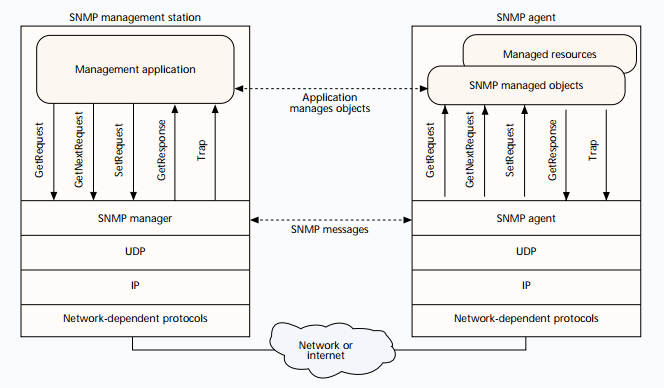
\includegraphics[width=0.5\textwidth]{snmp-arch}
  \end{center}
  \caption{The interaction between SNMP agent and management station\cite{Stallings1998}}
  \label{fig:snmp-arch}
\end{figure}

\subsection{Usage on constrained devices} % (fold)
\label{ssub:usage_on_constrained_devices}
The wide adoption of SNMP makes it an obvious candidate for IoT network management. This would enable existing tools to manage IoT-nodes without modifications. SNMP was designed to focus on simplicity and minimize the overhead needed to run it, in order to make it usable on as many systems as possible. However, it was not designed for hard constraints as described in section~\ref{sub:requirements_introduced_by_the_internet_of_things}, so it needs to be investigated which hardware is the bottom line still able to run SNMP.

The authors of \cite{mgmt-constrained-iot} have tried to answer this question by implementing  SNMP on the Atmel AVR Raven, a constrained device roughly translating to class 1 as defined in section~\ref{sub:requirements_introduced_by_the_internet_of_things}, running Contiki OS \cite{Dunkels2004}. They found that ``SNMP makes efficient use of resources on constrained devices''~\cite{mgmt-constrained-iot}, using between six and 24 percent of ROM and less than one percent of RAM, depending on the version of SNMP enabled.

\begin{table}[h]
\begin{tabular}{|l|l|l|l|}
\hline
\textbf{Component} & \textbf{RAM} & \textbf{ROM} & \textbf{Stack} \\ \hline
SNMPv1+SNMPv3/USM  & 235 (1\%)    & 31220 (24\%) & 1144 (7\%)     \\
SNMPv1             & 43 (0.2\%)   & 8860 (6\%)   & 688 (4\%)      \\
NETCONF            & 627 (4\%)    & 22768 (17\%) & 678 (4\%)      \\
TLS Total          & 1861 (11\%)  & 37440 (29\%) & 1834 (11\%)    \\
DTLS Total         & 1961 (12\%)  & 37232 (28\%) & 2454 (15\%)    \\ \hline
\end{tabular}
\label{table:snmp-netconf-constrained-implementation}
\caption{Comparison of memory usage on an AVR Raven\cite{mgmt-constrained-iot}}
\end{table}

The same implementation was able to process SNMP requests in 40-120 ms, depending on the used version of SNMP and the chosen security level, as illustrated in figure~\ref{fig:snmp-processing-time}. 

\begin{figure}[h]
  \begin{center}
    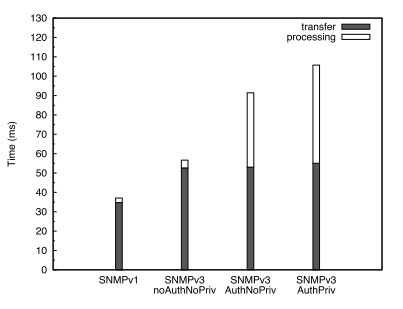
\includegraphics[width=0.5\textwidth]{snmp-processing-time}
  \end{center}
  \caption{Average processing and transfer time of SNMP~\cite{mgmt-constrained-iot}}
  \label{fig:snmp-processing-time}
\end{figure}

It remains unclear though how well SNMP is able to cope with the limitations of constrained networks such as high packet loss and low throughput. Besides that the impact on energy consumption is not evaluated yet, while being a major limitation in the IoT. Further experiments should be conducted to answer these questions.

Another approach to incorporate SNMP in IoT management is the use of a proxy to translate SNMP requests into a protocol designed for usage in constrained environments. This would maintain compatibility with existing management tools using SNMP while making it unnecessary to the problems of its usage on constrained devices. The authors of~\cite{Lindholm-Ventola2014} have developed a prototype for this approach using the Constrained Application Protocol (CoAP)~\cite{draft-ietf-core-coap-18} for communication from the constrained network to the gateway. CoAP is an application layer protocol designed by the IETF Constrained RESTful Environments (CoRE) working group. It translates easily to HTTP and uses UDP and 6LoWPAN~\cite{rfc4919}, an adaptation layer for usage of IPv6 on constrained devices. The gateway prototype uses CoAP to retrieve information from a constrained network and provides this as an SNMP agent.

As a conclusion it can be stated that the wide adoption of SNMP makes it worthwile to conduct further research on the feasability of its usage in the IoT. Existing prototypes show that SNMP uses resources efficiently, but it is an open question how it would behave in a real-world scenario.

% subsubsection usage_on_constrained_devices (end)

% subsection snmp (end)


\subsection{Netconf/Yang} % (fold)
\label{sub:netconf_yang}
The Network Configuration Protocol (NETCONF) is a network management protocol first published in 2006~\cite{rfc4741} and revised in 2011~\cite{rfc6241}. The intention was to develop a better protocol for device configuration, after realizing that SNMP is often used for network monitoring only while proprietary interfaces are used for configuration.

Compared to SNMP NETCONF puts less emphasis on simplicity, using XML based encoding and connection-oriented delivery over TCP, with mandatory security mechanisms such as SSH. Instead it aims to provide a feature-complete solution for network management in order to make this unified approach more attractive than proprietary solutions.

Configuration and state data is described in the YANG~\cite{rfc6020} data modeling language, which is based on XML. NETCONF has the capability to ``install, manipulate, and delete the configuration of network devices''~\cite{rfc6241}.


\subsection{Usage on constrained devices } % (fold)
\label{ssub:usage_on_constrained_devices_}
In the experiment referenced in~\ref{ssub:usage_on_constrained_devices} a prototype implementation of NETCONF has been tested on the same device and compared to the SNMP implementation~\cite{mgmt-constrained-iot}. The results can be seen in table~\ref{table:snmp-netconf-constrained-implementation}, showing that consumption of RAM and ROM is an order of magnitude higher than SNMP. The processing time of simple requests is significantly increased as well at 500 to 900 ms, which is up to 22 times longer than SNMP. The authors attribute this to the overhead necessary for processing XML, taking 80 to 90 percent of the total processing time for major operations. They note that this could be significantly improved by using an optimized XML library using less write operations. 

The second major problem identified by the authors occurs when adding a security layer to NETCONF operations. In this case TLS was used, adding a delay in the order of seconds when starting a session. This problem could be mitigated by using hardware encryption support, however constrained devices usually lack this type of hardware. 

NETCONF uses TCP for data transmission, which is not considered a good fit for unreliable, low-throughput wireless transmissions. TCP ensures reliable transmission after establishing a connection, as opposed to UDP which enables a best-effort transmission without setup of an end-to-end connection. The acknowledgement and retransmission required for reliable transmission causes increased load on the network nodes, thus increasing energy consumption and decreasing throughput~\cite{Dunkels2003}. Overall TCP causes a significant overhead for constrained devices. 

A proposal of RESTful interfaces for data defined in YANG~\cite{Bierman} might provide a more resource friendly alternative to the data transfer in NETCONF. The use of compact encoding of RESTful APIs in CoAP would reduce the message size by:

\begin{itemize}
  \item Avoiding TCP session overhead
  \item Reducing HTTP verbosity
  \item Using JSON instead of XML
\end{itemize}

It should be noted that the impact of security mechanisms remains unchanged, since CoAP uses DTLS for transport-layer security which shares most of the underlying cryptography with TLS.

Another proposal aimed to make an implementation of NETCONF on constrained devices feasible is NETCONF Light (NCL)~\cite{Perelman}. The main idea of this draft is reducing complexity via modularization, making it possible for a device to announce that it only implements a subset of NETCONF functionality. This will likely result in reduced memory usage and size of code base.

To summarize, many aspects in the design of NETCONF are not well suited for constrained devices but an effort is made to overcome these difficulties. It remains unclear if these proposed changes will be realized. The general viability of a NETCONF implementation on constrained devices has been shown, but it is an open question how this translates to a real-world scenario. The tradeoff between increased management capabilities and reliable transmission to efficient use of resources has to be evaluated for IoT networks.

% subsubsection usage_on_constrained_devices_ (end)

% subsection netconf_yang (end)


\section{Network Management Approaches for the IoT} % (fold)
\label{sec:network_management_approaches_for_the_iot}
Section~\ref{sec:traditional-nm} has introduced existing network management protocols and their adaptations to constrained devices. The protocols introduced in the following are specifically designed for use in the IoT.
\subsection{CoAp Management Interfaces} % (fold)
\label{sub:comi}
The CoAp Management Interfaces (CoMI) draft~\cite{draft-vanderstok-core-comi-04} describes a way to adapt REST-based protocols developed for constrained node networks to SNMP-based network management.
CoMI uses CoAP for data transmission, which is designed to easily translate to HTTP in constrained environments, as described in~\ref{ssub:usage_on_constrained_devices}. The data is encoded in the Concise Binary Object Representation~\cite{rfc7049}, a binary data format aimed to allow compact serialization of common data types. The underlying data model of CBOR is based on the JSON data model, thus conversion between these data formats is easy by design. 

The rationale to this approach is to prevent adding a second application layer protocol to constrained devices, assuming that CoAP and CBOR implementations are already present. Another obvious advantage is the efficient usage of resources by utilizing protocols and data types designed specifically for this environment, even though SNMP is reasonably efficient in this regard as outlined in section~\ref{ssub:usage_on_constrained_devices}.

The main challenge for CoAP is the mapping of SNMP-based MIBs encoded in SMIv2~\cite{rfc2578} to a CBOR representation. One possible pipeline to achieve this is as follows~\cite{Bergmann}:

\begin{enumerate}
  \item Conversion from SMIv2 to YANG-structured data
  \item Translation to JSON using data-model driven XML to JSON translation~\cite{rfc6110}
  \item Translation from JSON to CBOR is trivial
\end{enumerate}

The authors of~\cite{Bergmann} note that this approach still requires transfer of the identifiers from the constrained nodes, leading to increased network traffic and the requirement to store those identifiers on the constrained nodes. They propose usage of the numerically structured Object ID defined in SMIv2-based MIBs and further simplification by factoring out common prefixes. In the presented example the unfactored CBOR representation is not significantly smaller than the original encoding, whereas the factored representation is about 70 percent smaller.

A problem for the adoption of CoMI is the relatively early stage of its development. The protocol is in the status of an Internet-Draft at the time of this writing. The working document is in active development, with the latest draft submitted only weeks ago\cite{draft-vanderstok-core-comi-04}. A published implementation of the protocol is not known to the auhor.

To summarize, CoMI is a promising approach because it maintains compatibility to existing management solutions while using specialized IoT protocols. The used protocols fit relatively well to SNMP and related datastructures. The early stage of development is an inhibitor to widespread adoption at this point.



% subsection comi (end)
% section network_management_approaches_for_the_iot (end)

\subsection{LWM2M} % (fold)
\label{sub:lwm2m}
The Lightweight Machine to Machine (LWM2M) Protocol is a service and device management protocol specified by the Open Mobile Alliance (OMA), a standards development organization for the mobile phone industry~\cite{yucianga-lwm2m}. An open source implementation of LWM2M is developed at the Eclipse Foundation under the name ``Wakaama''~\cite{eclipse-wakaama}.

LWM2M utilizes typical IoT technologies such as CoAP for data transmission and DTLS as a security layer. A differentiator to other protocols is the possibility to use SMS in the transport layer instead of TCP. The protocol stack of LWM2M is presented in table~\ref{fig:lwm2m-stack}.

\begin{table}[h]
\begin{center}
  \begin{tabular}{|c|c|}
  \hline
  \multicolumn{2}{|c|}{\textbf{LWM2M Objects}}  \\ \hline
  \multicolumn{2}{|c|}{\textbf{LWM2M Protocol}} \\ \hline
  \multicolumn{2}{|c|}{\textbf{CoAP}}           \\ \hline
  \multicolumn{2}{|c|}{\textbf{DTLS}}           \\ \hline
  \textbf{UDP}           & \textbf{SMS}         \\ \hline
  \end{tabular}
\end{center}

\caption{The protocol stack of LWM2M}
\label{fig:lwm2m-stack}
\end{table}


As implied by its name LWM2M puts an emphasis on machine to machine communication, while using lightweight protocols in order to be compatible to constrained devices. It is divided into three components:

\begin{enumerate}
  \item The bootstrap server for initial configuration of managed nodes
  \item A central server that manages all LWM2M clients
  \item Clients which execute operations assigned by the server and report results of these operations back to the server
\end{enumerate}

The interfaces between the components are defined as follows:

\begin{LaTeXdescription}
  \item [Device discovery and registration:] The client announces its existence to the server and advertises its capabilities.
  \item [Bootstrap:] The client receives its initial configuration from the bootstrap server. 
  \item [Device management and service enablement:] The server enables M2M services over this interface. Operations can be send to the client and the response indicates its result.
  \item [Information Reporting:] Clients can use this interface to report status information to the server. This can be performed periodically or triggered by events.
\end{LaTeXdescription}

The main differentiator of this architecture is the integration of service discovery into the management process. This enables automatic configuration as outlined in section~\ref{sub:service_and_device_discovery}. For example, a new device would use the service discovery and registration interface to announce its existence to the server. In the next step it can receive its initial configuration from the bootstrap server. At this point the device is ready for operation, can report its status to the LWM2M server and receive updated configuration.

The obvious disadvantage of this architecture is the use of a centralized server for management. This requires additional effort to set up and introduces a single point of failure. Apart from this it would be desirable to allow interaction with multiple management entities instead of binding a constrained device to a centralized  authority.

% subsection lwm2m (end)


\subsection{Message Queueing Telemetry Transport} % (fold)
\label{sub:mqtt}
Message Queuing Telemetry Transport (MQTT) is a lightweight messaging protocol implementing the publish-subscribe paradigm~\cite{mqtt}. 

Publish-subscribe describes an interaction scheme where messages are not sent directly to the receivers interested in them. Instead, subscribers can express interest in a class of events and will subsequently be notified of any such event. Publishers broadcast their respective information and it is forwarded to all subscribers interested in this class of information~\cite{Eugster2003}. This approach enables a loose coupling of publishers and subscribers, i.e. publishers do not need to maintain any information about their subscribers and vice-versa.

MQTT uses a broker as an intermediary between publisher and subscriber to realize this messaging scheme. Publishers send a \textit{pub} message to the broker, containing the data to be publish alongside the related topic. Subscribers send a \textit{sub} message to the broker containing the topic they are interested in. If the topic of \textit{sub} and \textit{pub} match the broker forwards the \textit{pub} message to the subscriber.

MQTT itself is not designed for use with constrained devices and some of its properties are not well suited for this kind of environment. In particular MQTT assumes a session-oriented, auto-segmenting point-to-point data transport service such as TCP/IP is provided by the network - this may not be the case on IoT nodes. However, MQTT-S is a publish-subscribe protocol based on MQTT developed for usage in wireless sensor networks. MQTT-S does not assume connection-oriented transport and does not rely on message segmentation or in-order delivery. Besides these reduced requirements MQTT-S defines a gateway to MQTT, allowing MQTT-S clients to be accessed like MQTT nodes. Figure~\ref{fig:mqtts-architecture} illustrates this architecture.

\begin{figure}[h]
  \begin{center}
    \includegraphics[width=0.5\textwidth]{mqtts-architecture}
  \end{center}
  \caption{MQTT-S Architecture~\cite{Hunkeler2008}}
  \label{fig:mqtts-architecture}
\end{figure}

MQTT and MQTT-S is not intended for network management as the previously introduced protocols, instead it provides an efficient way to distribute messages over a network. This can be used to implement network management tasks, an obvious example is the propagation of status information from the publishers. This approach should make significantly more efficient use of network resource compared to polling each node from a network management station.

As another advantage MQTT makes it superfluous to discover or advertise services, because they are managed by the broker. For example a network management station interested in the current battery load of nodes does not require any information about the nodes present in a network. Instead it simply subscribes to the related topic and subsequently receives status updates from all nodes in the network.

A disadvantage can be identified in the need for a broker in addition to the networking nodes, as well as the need for a gateway when using MQTT-S.

Apart from this the protocol lacks the universality of other network management protocols. Nodes have to be configured to use MQTT before deployment, and without further extensions it is not possible to change the mode of operation using MQTT. In comparison, all previously introduced network management solutions incorporate the ability to change the configuration of managed devices and this is an essential requirement of network management.

As a conclusion, MQTT makes efficient use of network resources and could be well suited for specialized tasks in the IoT. On the other hand, it lacks the universality of other protocols introduced in this work.


% subsection mqtt (end)

\section{Service Discovery} % (fold)
\label{sec:service_discovery}
As outlined in paragraph~\ref{sub:service_and_device_discovery}, service discovery is closely related to network management and often used in conjunction. The following paragraph will introduce commonly used protocols for service discovery and their applications to constrained devices.
% section service_discovery (end)


\subsection{DNS-based service discovery} % (fold)
\label{sub:dns_sd}
When implementing service discovery, the general approach is letting a service provider advertise the services it offers. Service consumers then query for a service they want to use and receive a list of the available service providers. The fundamental problem of this idea is the requirement of an intermediary which can be used for advertisement and storage.

Under the assumption that DNS is a bottom-line infrastructure available in all relevant networks, it can be utilized for DNS-based service discovery (DNS-SD)~\cite{rfc6763}. The procedure is exactly as outlined above - a service provider announces its existence in a special DNS resource record~\cite{rfc2782}. Consumers can browse this directory to identify consumable service providers and how to access them. To provide a specific use-case for network management, a network node running an SNMP agent could use SNMP-SD to advertise this capability and the available interfaces using DNS-SD~\cite{Tsou}.

The problem of this solution is its reliance on DNS infrastructure which may not be available in constrained networks.


% subsection dns_sd (end)

\subsection{Multicast DNS} % (fold)
\label{sub:mdns}
Multicast DNS (mDNS)~\cite{rfc6762} was developed to enable domain resolution in networks lacking a DNS infrastructure. This is implemented by using IP multicast to send DNS-like UDP queries and responses. Names are resolved from local resource records stored by each node.

Multicast DNS is commonly used in conjunction with DNS-SD to enable service discovery without additional DNS infrastructure. This creates a zero-configuration environment where devices can be initialized without previous configuration.

A prototype implementation of mDNS and DNS-SD on constrained devices~\cite{Siljanovski} proves that these protocols are generally usable in an IoT context.


% subsection mdns (end)

% An example of a floating figure using the graphicx package.
% Note that \label must occur AFTER (or within) \caption.
% For figures, \caption should occur after the \includegraphics.
% Note that IEEEtran v1.7 and later has special internal code that
% is designed to preserve the operation of \label within \caption
% even when the captionsoff option is in effect. However, because
% of issues like this, it may be the safest practice to put all your
% \label just after \caption rather than within \caption{}.
%
% Reminder: the "draftcls" or "draftclsnofoot", not "draft", class
% option should be used if it is desired that the figures are to be
% displayed while in draft mode.
%
%\begin{figure}[!t]
%\centering
%\includegraphics[width=2.5in]{myfigure}
% where an .eps filename suffix will be assumed under latex, 
% and a .pdf suffix will be assumed for pdflatex; or what has been declared
% via \DeclareGraphicsExtensions.
%\caption{Simulation Results}
%\label{fig_sim}
%\end{figure}

% Note that IEEE typically puts floats only at the top, even when this
% results in a large percentage of a column being occupied by floats.


% An example of a double column floating figure using two subfigures.
% (The subfig.sty package must be loaded for this to work.)
% The subfigure \label commands are set within each subfloat command, the
% \label for the overall figure must come after \caption.
% \hfil must be used as a separator to get equal spacing.
% The subfigure.sty package works much the same way, except \subfigure is
% used instead of \subfloat.
%
%\begin{figure*}[!t]
%\centerline{\subfloat[Case I]\includegraphics[width=2.5in]{subfigcase1}%
%\label{fig_first_case}}
%\hfil
%\subfloat[Case II]{\includegraphics[width=2.5in]{subfigcase2}%
%\label{fig_second_case}}}
%\caption{Simulation results}
%\label{fig_sim}
%\end{figure*}
%
% Note that often IEEE papers with subfigures do not employ subfigure
% captions (using the optional argument to \subfloat), but instead will
% reference/describe all of them (a), (b), etc., within the main caption.


% An example of a floating table. Note that, for IEEE style tables, the 
% \caption command should come BEFORE the table. Table text will default to
% \footnotesize as IEEE normally uses this smaller font for tables.
% The \label must come after \caption as always.
%
%\begin{table}[!t]
%% increase table row spacing, adjust to taste
%\renewcommand{\arraystretch}{1.3}
% if using array.sty, it might be a good idea to tweak the value of
% \extrarowheight as needed to properly center the text within the cells
%\caption{An Example of a Table}
%\label{table_example}
%\centering
%% Some packages, such as MDW tools, offer better commands for making tables
%% than the plain LaTeX2e tabular which is used here.
%\begin{tabular}{|c||c|}
%\hline
%One & Two\\
%\hline
%Three & Four\\
%\hline
%\end{tabular}
%\end{table}


% Note that IEEE does not put floats in the very first column - or typically
% anywhere on the first page for that matter. Also, in-text middle ("here")
% positioning is not used. Most IEEE journals/conferences use top floats
% exclusively. Note that, LaTeX2e, unlike IEEE journals/conferences, places
% footnotes above bottom floats. This can be corrected via the \fnbelowfloat
% command of the stfloats package.



\section{Conclusion}

This work has developed the requirements of network management in the Internet of Things and introduced existing solutions to evaluate their satisfaction of these requirements.

In general it can be stated that each of the presented protocols incorporates advantages and shortcomings compared to each other. At the same time none of the protocols can be seen as the single solution to solve all network management tasks in the internet of things.

One realization of this work is that existing protocols which are widely used outside of the IoT, namely SNMP and NETCONF, can be adapted to constrained devices. The advantage of using existing tools and systems for IoT management should be reason enough to consider further usage of these protocols. 

A special case in this regard is CoMI because it allows interoperability with existing SNMP infrastructure, thus the same argument can be made for it.

DNS based service discovery is an important enhancement to these protocols and existing research suggests that it can be adopted to constrained devices.

The remaining protocols MQTT and LWM2M are less ubiquitous in comparison but serve their respective niche very well.





% trigger a \newpage just before the given reference
% number - used to balance the columns on the last page
% adjust value as needed - may need to be readjusted if
% the document is modified later
%\IEEEtriggeratref{8}
% The "triggered" command can be changed if desired:
%\IEEEtriggercmd{\enlargethispage{-5in}}

% references section

% can use a bibliography generated by BibTeX as a .bbl file
% BibTeX documentation can be easily obtained at:
% http://www.ctan.org/tex-archive/biblio/bibtex/contrib/doc/
% The IEEEtran BibTeX style support page is at:
% http://www.michaelshell.org/t ex/ieeetran/bibtex/
\bibliographystyle{IEEEtran}
% argument is your BibTeX string definitions and bibliography database(s)
\bibliography{seminar_technische_informatik,rfc}
%





% that's all folks
\end{document}


